\subsection{Optimale speckle patterns} \label{Optimale speckle patterns}

Et godt speckle pattern er karakteriseret ved høj kontrast mellem prikker og baggrund, og et tilfældigt mønster, der er jævnt fordelt og udgør mellem 50\% og 70\% af billedet. Prikkerne skal have en ensartet radius, samt have en størrelse på mellem $3\times3$ og $5\times5$ pixels. Derudover skal prikkerne være indenfor kameraets field of view (FOV). I denne rapport referer FOV til længden af det område kameraet observerer, det er dermed en konsekvens af dets brændvidde og afstand til emnet. (\cite{Dong2017ACorrelation}; \cite{Su2022Glare:Pattern}; \cite{Gagnon2024ThePatterns}).  


%------
\subsubsection{Høj kontrast}\plainbreak{-0.4} 
DIC benytter gray-level til vurdering af prikkernes placering på overfladen. Gray-level er en grå-skala værdi fra 0\% til 100\%, der beskriver lysintensiteten i et enkelt pixel. Et gray-level på 100\% ses som hvid, hvor 0\% er helt sort, gray-level værdien angiver mængden af lys. Værdierne angives fra 0 til 255 for et 8-bit kamera. Det er nødvendigt med høj kontrast, så kameraet kan opfange forskellen mellem prikker og baggrund. Ofte bruges sorte prikker på hvid baggrund, eller hvide prikker på sort baggrund, idet disse har størst forskel mellem prikkerne og baggrundens gray-level. Forskellen mellem baggrund og prikker skal være på minimum 52 point, for at opnå en optimal værdi, skal denne forskel ligge på 130 point og derover (\cite{Reu2015AllContrast}; \cite{Bigger2018ACorrelation}).


%----- 
\newpage
\subsubsection{Størrelse på prikkerne} \plainbreak{-0.4}
Prikkernes størrelse har betydning for, hvordan prikkerne opfanges af kameraet, samt softwaren bearbejder dataen. For at opnå et optimalt resultat skal prikkerne være større end tre pixels, hvilket afhænger af kameraets opløsning og FOV. Den minimale diameter på prikkerne ($\diameter_{min}$), er derfor afhængig af FOV og antallet af pixels ($n_{pixels}$), som det fremgår af formel \ref{equ:prikstørrelse-Ø_min}. FOV definerer enten bredden eller højden på området, indenfor kameraets synsfelt, der er påført speckle pattern og måles i millimeter. Formlen bruges til at give et estimat, af den minimale diameter prikkerne må have, for at give et optimalt resultat ved DIC. $\diameter_{min}$ beregnes separat for henholdsvis bredden og højden af FOV. Hvis $\diameter_{min}$(bredden) $\neq \diameter_{min}$(højden), benyttes den største diameter (\cite{Reu2014AllAliasing}).
 \begin{equation} \label{equ:prikstørrelse-Ø_min}
     \diameter_{min} = \frac{FOV}{n_{pixels}} \cdot n_{min \ \vee \  max \ pixels} 
 \end{equation}
Prikker mindre end $3\times3$ pixels er vanskelige at bestemme centrum af, idet en prik på $1\times1$ pixels der ligger mellem to pixels vil give en slørret afbildning i gray-level, hvorved kontrasten mellem prik og baggrund mindskes, hvilket medfører en stigning i systematiske fejl. Yderligere øges præcisionen ved brug af prikker over $3\times3$ pixels, fordi det bliver tydeligere på gray-level, hvor prikken er lokaliseret, da den vil dække flere pixels, selvom prikken er placeret mellem to pixels, som det er illusreret på figur \ref{fig:gray-level}. (\cite{Reu2014AllAliasing}; \cite{Cui2024EffectError})

\begin{figure}[H]
    \centering
    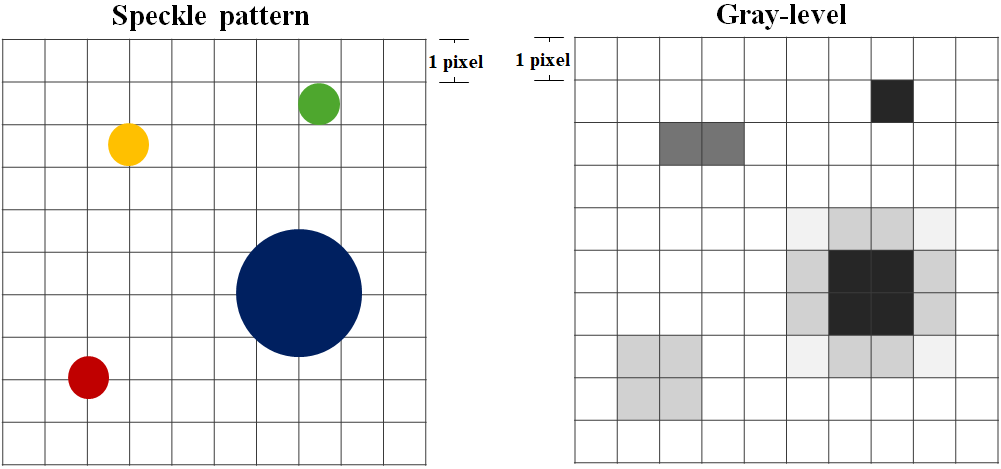
\includegraphics[width=0.8\linewidth]{Sections/2 Problemanalyse/Media/gray-level.png}
    \caption{Illustration af computersoftwares opfattelse af sepckel patterns. Gitteret illustreret et subset på $10\times10$ pixels. Den \textcolor{red}{røde}, \textcolor{greenB}{grønne} og \textcolor{gulny}{gule} prik er alle $1\times1$ pixels, placeret forskelligt i gitteret. Den \textcolor{blue}{blå} prik er $3\times3$ pixels.}
    \label{fig:gray-level}
\end{figure} \plainbreak{-.5}

Prikkerne kan ikke være uendeligt store, da de er begrænset af FOV, kameraets opløsning, det procentvise forhold prikkerne må dække af hele overfladen, samt størrelsen på overfladen der undersøges. Når prikker er større bliver softwaren nød til at gøre brug af tilsvarende større subsets for at garantere unikke subsets. Der skal altså findes et kompromis mellem størrelsen af subsets, dermed nøjagtighed, og systematiske fejl fra prikker placeret på kanten af pixels. Dette kompromis er en prikstørrelse på mellem $5 \times 5$ og $8 \times 8$ pixels. (\cite{Haddadi2008UseTechnique}; \cite{Crammond2013SpeckleCorrelation}; \cite{Dong2017ACorrelation};  \cite{Gagnon2024ThePatterns})


Ved forventning om store deformationer, hvor mindre deformationer er uvæsentlige at undersøge, kan større prikker bruges, uden det har betydning for det der ønskes undersøgt. Overfladens størrelse medvirker til den maksimale størrelse prikkerne kan have, idet store overflader, kan benytte prikker af en større størrelse til subsets, fordi FOV er større (se \ref{equ:prikstørrelse-Ø_min}). Prikkerne i det samme speckle pattern kan variere mellem tre pixels og otte pixels, men for optimal måling skal størrelsesforskellen på prikkerne i det samme speckle pattern holdes minimal(\cite{Crammond2013SpeckleCorrelation}; \cite{Gagnon2024ThePatterns}).  

%-----
\subsubsection{Tilfældigt og isotropt}\plainbreak{-0.4}
Identifikationen af et subset's bevægelse efter deformation af emnet, er kun mulig, hvis prikkerne er arrangeret i et mønster der ikke gentages. Hvis de ligger på linje er det ikke muligt at se hvis prikkerne er forskudt langs den linje (\cite{Zaya2023ApplicationReview}).

%----
\subsubsection{Fordeling af prikkerne}\plainbreak{-0.4}
Et godt speckle pattern har en 50\% til 70\% dækning af prikker. Prikkerne skal være jævnt fordelt med minimum tre pixels mellem alle prikkerne. Hvis prikkerne er for tætte på hinanden, kan softwaren have det vanskeligt med at identificere, om det er én stor prik eller flere små prikker, hvilket øger usikkerheden ved måling. (\cite{Reu2015AllDensity}; \cite{Caliskan2024InvestigationDIC})

\begin{figure}[H]
  \centering
    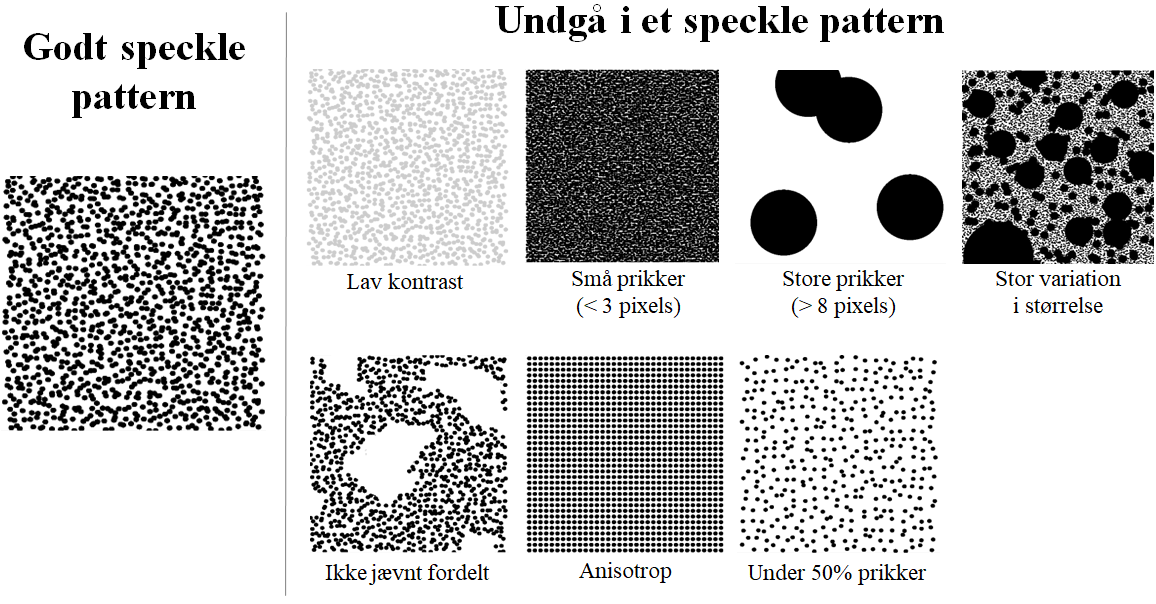
\includegraphics[width=0.9\textwidth]{Sections/2 Problemanalyse/Media/speckle pattern.png}
    \caption{Illustration af fejlkilder ved produktion af speckle pattern til DIC. Speckle pattern er genereret med software fra Correlated Solutions (\cite{CorrelatedSolutions2025SpeckleInc.})}
    \label{fig:godt speckle pattern}
\end{figure} \plainbreak{-0.4}

Figur \ref{fig:godt speckle pattern} illustrerer fejlkilder i speckle patterns, der mindsker præcisionen af DIC. Kriterierne for et godt speckle pattern er gældende for både 2D og 3D.


%-----
\subsubsection{Forblive på overfladen} \plainbreak{-0.4}
Det er nødvendigt, at prikkerne forbliver på og deformerer med overfladen af emnet der undersøges. Resultaterne af DIC er ikke retvisende, hvis prikkerne flytter sig uafhængigt af det undersøgte emne. Det er nødvendigt, at prikkerne flytter sig med emnet og ikke påvirker dets egenskaber. Derudover skal prikkerne ikke have tydelig ændring i gray-level eller geometri efter deformation.
(\cite{Dong2017ACorrelation} ; \cite{Zaya2023ApplicationReview}). \label{par:overfladen}

